% Probably doesn't justify a separate section. Most people do not have it.

% Need more explanation with designs for both generalisation and atomisation.
% Including limitations.

\chapter{Implementation}

In this section, the architecture of the entire concept bottleneck pipeline, as well as more detail unrelated to logical modelling, is presented.
Since, the work in this thesis is a continuation of the previous unpublished work, laid out in \autoref{inherited-work}, this section may include some parts which do not constitute my work. 
The * sign is used to signify the work that is not the work of the author of the thesis.


\section{Concept Bottleneck Pipeline*}

% TODO: fix X in picture, add boxes for the three parts, missing outlining X as attention module
\begin{figure}[h]
\caption{The full pipeline for the classification of MLB-V2E dataset using concept bottleneck model (adapted from \cite{RefWorks:RefID:16-2021automatic})}
\centering
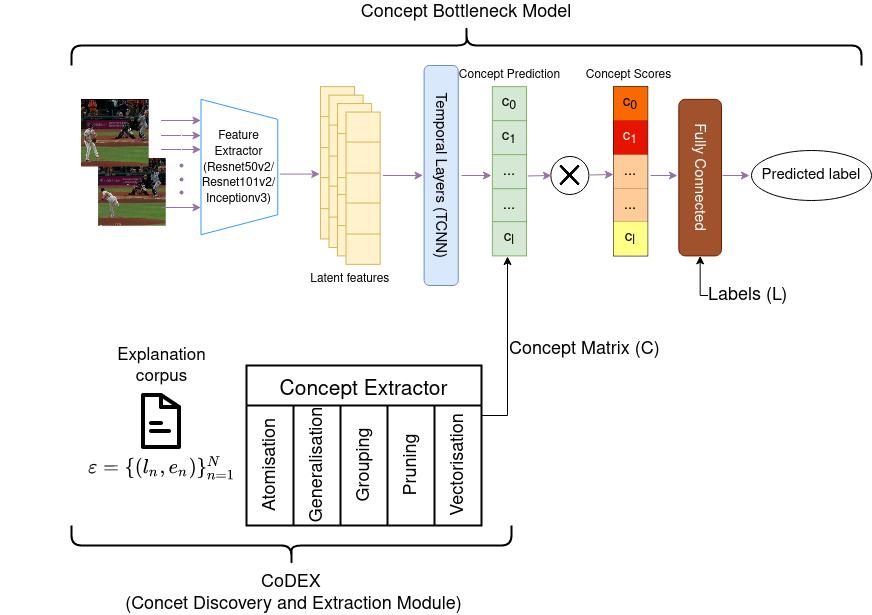
\includegraphics[width=\textwidth]{implementation/full architecture diagram.png}
\label{full-architecture-diagram}
\end{figure}

The concept bottleneck pipeline is shown in \ref{full-architecture-diagram}. 
Its purpose is to predict an output label correctly and in an interpretable manner.
The pipeline can be divided into concept extraction, concept prediction and label prediction pipeline. \\

\textbf{Concept Discovery and Extraction Pipeline (CoDEx)} is used to find an informative set of concepts for the problem at hand.
These concepts are extracted using human-generated explanations and labels in the dataset. 
The module consists of 5 parts: atomisation, generalisation, grouping, pruning, and vectorisation.

% INSERT chapter to reference.
The first two will be explained further in section X, while the latter 3 have been kept the same as explained in \autoref{inherited-work}. \\


\textbf{Concept Prediction Pipeline} has to predict the extracted concepts for the training images and varies depending on the problem type dealt with.
In all cases, it is a multi-label prediction model where output labels are probabilities that raw concepts occur.
The true labels for training are obtained from the concept matrix returned by the CoDEx module. \\

\textbf{Label Prediction Pipeline} has to predict the final output labels from the derived concepts. 
It consists of the attention mechanism, which highlights more relevant concepts for the prediction, and the fully connected layers. 
For further interpretability, the fully connected layer might be replaced with a neuro-symbolic component as a part of a future work.

\subsection{Dependencies}

\textbf{Sentence Transformers}: A library which provides access to pre-trained transformers. 
Since it is only used in the grouping stage, the ease of use of the library was the main reason for the selection of the library.


Finally, \textbf{numpy}, \textbf{scikit-learn}, \textbf{matplotlib}, \textbf{panadas} which all are famous Python libraries used with AI projects. \\
